\section{CHƯƠNG 4: TIỀN XỬ LÝ DỮ LIỆU VÀ RÚT TRÍCH ĐẶC TRƯNG} \label{sec:dep_fe}

\subsection{Giới thiệu chung}

Chương này trình bày chi tiết quy trình khám phá, tiền xử lý tập dữ liệu thô thu thập được từ TikTok và các bước rút trích đặc trưng cần thiết. Mục tiêu của quá trình này là chuẩn bị một tập dữ liệu sạch, có cấu trúc tốt và giàu thông tin, sẵn sàng cho các giai đoạn phân tích sâu hơn và làm cơ sở cho việc xây dựng công cụ hỗ trợ viết kịch bản video TikTok.

Dữ liệu thô thu thập được bao gồm hai tập chính: \textbf{dữ liệu về video TikTok} (thông tin chi tiết của từng video như lượt xem, thích, chia sẻ, bình luận, v.v.) và \textbf{dữ liệu về người dùng TikTok} (thông tin về tài khoản người đăng như số lượng người theo dõi, video đã đăng, v.v.).

\textbf{Trong chương này, nhóm sẽ tập trung trình bày chi tiết các bước khám phá, tiền xử lý và rút trích đặc trưng đối với tập dữ liệu video TikTok}. Lý do là vì quy trình xử lý dữ liệu trên tập người dùng cũng bao gồm nhiều bước tương đồng với dữ liệu video. \textbf{Do đó, chi tiết về quá trình tiền xử lý dữ liệu người dùng sẽ không được trình bày cụ thể tại đây mà có thể được tìm hiểu kỹ hơn trong file Jupyter Notebook} trong link GitHub của nhóm.

Quy trình xử lý chung được áp dụng (đặc biệt trên dữ liệu video) bao gồm các bước chính như tìm hiểu cấu trúc và đặc điểm dữ liệu thô, xử lý các giá trị bị thiếu và trùng lặp, chuẩn hóa kiểu dữ liệu, loại bỏ các cột không cần thiết, và cuối cùng là tạo ra các đặc trưng mới từ dữ liệu văn bản và thời gian để làm giàu tập dữ liệu.

\subsection{Khám phá và Tiền xử lý dữ liệu (Data Exploration and Preprocessing - DEP)}

Quá trình tiền xử lý dữ liệu được thực hiện chủ yếu dựa trên phân tích trong file \texttt{02\_DEP\_01-\\Preprocess\_video\_data.ipynb}.

\subsubsection{Tìm hiểu tập dữ liệu thô}

\paragraph{Đọc dữ liệu:}
Tập dữ liệu thô (\texttt{final\_raw\_videos.csv}) được đọc vào DataFrame của Pandas. Ngay từ bước này, kiểu dữ liệu của một số cột đặc biệt (ví dụ: các cột ID, cột chứa giá trị dạng phân loại) đã được xác định trước là \texttt{object} (chuỗi) thay vì \texttt{int} (số nguyên) để tránh việc Pandas tự động nhận diện sai và phù hợp hơn với bản chất dữ liệu (không thực hiện phép toán số học trên các cột này).

\paragraph{Kích thước dữ liệu:}
Tập dữ liệu thô ban đầu bao gồm \textbf{71260 hàng} và \textbf{174 cột}.

\paragraph{Ý nghĩa dữ liệu:} 
Mỗi hàng trong tập dữ liệu đại diện cho thông tin thống kê và siêu dữ liệu (metadata) của một video TikTok thuộc chủ đề ẩm thực. Các cột bao gồm nhiều thông tin đa dạng như:
\begin{itemize}
    \item \textbf{Thông tin về tác giả:} tên, ID, số liệu thống kê như lượt theo dõi, lượt thích, v.v..
    
    \item \textbf{Thông tin về video:} ID, mô tả, thời gian tạo, lượt xem, lượt thích, bình luận, v.v..
    
    \item \textbf{Thông tin kỹ thuật:} thời lượng, độ phân giải, codec, v.v..
    
    \item \textbf{Thông tin về âm nhạc sử dụng:} tên bài hát, tác giả, v.v..
    
    \item \textbf{Các tính năng tương tác đặc biệt của TikTok} như \texttt{duet}, \texttt{stitch}, v.v..
    
    \item Và còn nhiều thông tin khác.
\end{itemize}

\subsubsection{Phân tích và xử lý dữ liệu trùng lặp (Duplicate Analysis)}

\paragraph{Xác định video:} 
Việc xác định các video trùng lặp dựa trên các cột ID (chứa mã định danh duy nhất) của video trong tập dữ liệu. Các cột này bao gồm: \texttt{id}, \texttt{video.id}, và \texttt{video.videoID}.

\paragraph{Xử lý các video bị thiếu ID:}
Phân tích cho thấy có \textbf{264 hàng} bị thiếu giá trị ở cả 3 cột ID này (chiếm 0.37\%). Do không thể xác định định danh duy nhất cho các video này, chúng đã bị loại bỏ khỏi tập dữ liệu. Tập dữ liệu sau khi loại bỏ còn \textbf{70996 hàng}.

\paragraph{Kiểm tra trùng lặp:}
Sử dụng cột \texttt{video.id} làm khóa chính để kiểm tra các hàng trùng lặp (giữ lại bản ghi đầu tiên nếu có trùng). Kết quả cho thấy \textbf{không có hàng nào bị trùng lặp} (tỷ lệ trùng lặp 0.00\%).

\begin{table}[H]
\centering
\caption{Thống kê dữ liệu ban đầu}
\begin{tabular}{lc}
\toprule
\textbf{Thông số} & \textbf{Giá trị} \\
\midrule
Số hàng ban đầu & 71.260 \\
Số cột ban đầu & 174 \\
Số hàng thiếu ID & 264 (0,37\%) \\
Số hàng sau loại bỏ & 70.996 \\
Tỷ lệ trùng lặp & 0,00\% \\
\bottomrule
\end{tabular}
\end{table}

\subsubsection{Phân tích và xử lý giá trị bị thiếu (Missing Value Analysis)}

\paragraph{Phân tích tỷ lệ thiếu:}
Biểu đồ phân bố tỷ lệ thiếu giá trị (Hình~\ref{fig:dep_missing_rate}) cho thấy một số lượng lớn các cột (khoảng 50\% tổng số cột) có tỷ lệ thiếu giá trị rất cao, \textbf{vượt quá 66.67\%} (thiếu hơn 2/3 dữ liệu).

\paragraph{Loại bỏ cột thiếu nhiều:}
Các cột có tỷ lệ thiếu trên 66.67\% được xem là không đủ chất lượng để phân tích và đã bị loại bỏ. Tổng cộng \textbf{87 cột} đã bị loại bỏ khỏi tập dữ liệu, giảm số lượng cột từ 174 xuống còn 87. 

\begin{figure}[H]
    \centering
    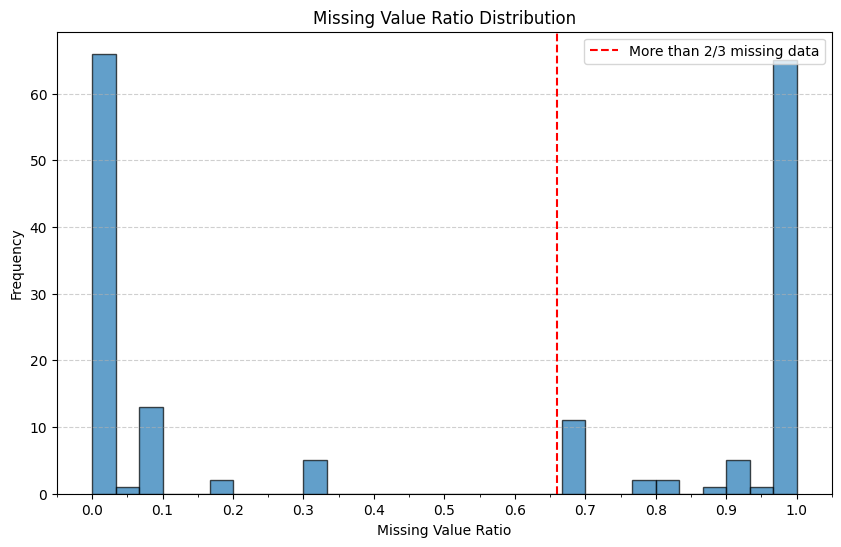
\includegraphics[width=.96\linewidth]{img/21127739/dep_missing_rate.png}
    \caption{Biểu đồ phân bố tỷ lệ thiếu giá trị của các cột}
    \label{fig:dep_missing_rate}
\end{figure}

\subsubsection{Phân tích và chuẩn hóa kiểu dữ liệu}

\paragraph{Kiểm tra kiểu dữ liệu:}
Sau khi loại bỏ các cột thiếu nhiều, kiểu dữ liệu của các cột còn lại được kiểm tra lại.

\paragraph{Chuẩn hóa cột thời gian:}
Hai cột \texttt{collectTime} (thời gian thu thập dữ liệu) và \texttt{createTime} (thời gian video được đăng tải) ban đầu có kiểu \texttt{object} và chứa giá trị dạng timestamp. Chúng đã được chuyển đổi sang kiểu \texttt{datetime} bằng hàm \texttt{pd.to\_datetime} với đơn vị là giây (\texttt{unit='s'}). Sau đó, múi giờ được chuẩn hóa về \textbf{GMT+7 (Asia/Ho\_Chi\_Minh)} để phù hợp với bối cảnh dữ liệu tại Việt Nam.

\vietnameselst
\begin{lstlisting}[language=Python]
# Convert the `collectTime` and `createTime` columns
# from POSIX to datetime64[ns] data type
video_df["collectTime"] = pd.to_datetime(video_df["collectTime"], unit="s")
video_df["createTime"] = pd.to_datetime(video_df["createTime"], unit="s")

# Change the timezone of the `collectTime` and `createTime` columns
# from UTC to Asia/Ho_Chi_Minh
video_df['createTime'] = video_df['createTime'].dt.tz_localize(
    'UTC').dt.tz_convert("Asia/Ho_Chi_Minh")
video_df['collectTime'] = video_df['collectTime'].dt.tz_localize(
    'UTC').dt.tz_convert("Asia/Ho_Chi_Minh")
\end{lstlisting}

\subsubsection{Phân tích phân bố giá trị}

\paragraph{Cột dạng số (Numerical):}
Phân tích thống kê mô tả (min, Q1, median, Q3, max) cho các cột số. Các nhận xét chính:
\begin{itemize}
    \item \texttt{authorStats.heart} và \texttt{authorStats.heartCount} có phân bố giống hệt nhau, cho thấy sự trùng lặp thông tin.
    
    \item Các cột \texttt{stats.*} và \texttt{statsV2.*} chứa thông tin tương tự (lượt xem, thích, bình luận, v.v.).
    
    \item Các cột \texttt{authorStats.friendCount} và \texttt{statsV2.repostCount} chỉ chứa một giá trị duy nhất (0.0), không mang lại nhiều thông tin biến thiên.
\end{itemize}

\paragraph{Cột không phải dạng số (Non-numerical):}
Phân tích số lượng giá trị duy nhất và tỷ lệ xuất hiện của từng giá trị. Nhận xét chính:
\begin{itemize}
    \item Nhiều cột chỉ chứa \textbf{1 giá trị duy nhất} (ví dụ: \texttt{author.commentSetting} chỉ có giá trị `0.0', \texttt{author.ftc} chỉ có `False', v.v.). Các cột này không hữu ích cho việc phân tích sự khác biệt giữa các video.
\end{itemize}

\subsubsection{Loại bỏ các cột không cần thiết/trùng lặp}

Dựa theo các phân tích trước đó, ta tiếp tục loại bỏ các cột không có nhiều ý nghĩa trong quá trình phân tích. Các cột được loại bỏ bao gồm:
\begin{itemize}
    \item \textbf{Cột ID trùng lặp}: Loại bỏ \texttt{id} và \texttt{video.videoID}, giữ lại \texttt{video.id} làm định danh chính cho video.
    
    \item \textbf{Cột thống kê cũ}: Loại bỏ các cột bắt đầu bằng \texttt{stats.*} (ví dụ: \texttt{stats.collect-\\Count}) vì trùng lặp với \texttt{statsV2.*}.
    
    \item \textbf{Cột có một giá trị duy nhất}: Loại bỏ 25 cột như \texttt{author.commentSetting}, \texttt{collected}, v.v. vì không cung cấp nhiều thông tin để phân tích.
    
    \item \textbf{Cột liên quan đến ngôn ngữ}: Loại bỏ các cột về ngôn ngữ video (ví dụ: \texttt{video.cla-\\Info.originalLanguageInfo.*}), vì dữ liệu tập trung vào khán giả Việt Nam.
    
    \item \textbf{Cột `heart' trùng lặp}: Loại bỏ \texttt{authorStats.heart} do trùng thông tin với \texttt{author-\\Stats.heartCount}.
\end{itemize}

Tổng cộng, \textbf{37 cột được loại bỏ}, giảm số lượng cột từ 87 xuống còn 50. Quá trình này được thực hiện bằng cách sử dụng các hàm phân tích của \texttt{Pandas}, như kiểm tra số giá trị duy nhất và so sánh phân phối giữa các cột.

\subsubsection{Xử lý dữ liệu thiếu trong các cột còn lại}

Đối với 50 cột còn lại, nhóm tiến hành xử lý dữ liệu thiếu như sau:
\begin{itemize}
    \item \textbf{Cột số}: Dữ liệu thiếu được điền bằng \textbf{giá trị trung vị} của cột, đảm bảo không làm lệch phân phối dữ liệu.
    \item \textbf{Cột không phải số}: Dữ liệu thiếu được điền bằng \textbf{giá trị đặc biệt} ``\texttt{others}'', tránh gây nhiễu trong phân tích.
\end{itemize}

Quá trình này đảm bảo không còn giá trị thiếu trong tập dữ liệu, với thông tin được xác nhận bằng phương thức \texttt{info()} của \texttt{Pandas}.

\subsubsection{Lưu trữ dữ liệu đã xử lý}

Kết thúc quá trình tiền xử lý, tập dữ liệu đã được làm sạch, chuẩn hóa, không còn giá trị thiếu và có kích thước \textbf{70996 hàng x 50 cột}. Kiểu dữ liệu của các cột đã phù hợp. Tập dữ liệu này được lưu dưới định dạng Parquet vào file \texttt{preprocessed\_videos.parquet} và sẵn sàng cho bước rút trích đặc trưng.

\subsection{Rút trích đặc trưng (Feature Engineering - FE)}

Sau khi làm sạch dữ liệu, nhóm tiến hành rút trích các đặc trưng quan trọng để hỗ trợ phân tích nội dung video và xây dựng công cụ viết kịch bản. Các đặc trưng bao gồm hashtag, nội dung video hàng đầu, transcript audio, thông tin món ăn, địa điểm và phân loại video.

\subsubsection{Trích xuất hashtag từ mô tả video (\texttt{desc})}

\paragraph{Quy trình:}
Từ cột \texttt{desc} chứa mô tả video, ta sử dụng biểu thức chính quy (thư viện \texttt{re} trong Python) để tìm và trích xuất các hashtag (chuỗi bắt đầu bằng ký tự \texttt{\#}). Các hashtag được chuẩn hóa bằng cách chuyển thành chữ thường và loại bỏ các dấu câu ở cuối (nếu có), đồng thời chuyển thành dạng không dấu (sử dụng thư viện \texttt{unidecode}).

\paragraph{Đặc trưng mới:}
\begin{itemize}
    \item \texttt{hashtags}: Một cột mới chứa danh sách (list) các hashtag đã được chuẩn hóa cho mỗi video.
    
    \item \texttt{hashtag\_count}: Một cột mới chứa số lượng hashtag có trong mỗi video.
\end{itemize}

\paragraph{Phân tích:}
Bảng~\ref{tab:hashtag_stats} cho thấy có đến \textbf{99,51\%} video (70.650/70.996) được đăng tải chứa ít nhất một hashtag, với trung bình \textbf{6-7 hashtag mỗi video}. Bảng~\ref{tab:popular_hashtags} cho thấy các hashtag phổ biến nhất bao gồm \texttt{ancungtiktok}, \texttt{learnontiktok}, \texttt{reviewanngon}, \texttt{xuhuong}, \texttt{mukbang}, phù hợp với chủ đề ẩm thực và xu hướng chung trên TikTok.

\begin{table}[H]
\centering
% Create two minipages side by side with vertical separator
\begin{minipage}[t]{0.47\textwidth}
    \centering
    \caption{Kết quả thống kê về hashtag}
    \label{tab:hashtag_stats}
    \renewcommand{\arraystretch}{1.3}
    \setlength{\tabcolsep}{4pt}
    \begin{tabular}{l}
    \toprule
    Total number of videos: \textbf{70996} \\
    Videos with hashtags: \textbf{70650} \\
    Percentage with hashtags: \textbf{99.51\%} \\
    Average hashtags per video: \textbf{6.85} \\
    \bottomrule
    \end{tabular}
\end{minipage}%
\hspace{0.01\textwidth}\vrule\hspace{0.01\textwidth}%
\begin{minipage}[t]{0.47\textwidth}
    \centering
    \caption{Danh sách các hashtag phổ biến}
    \label{tab:popular_hashtags}
    \renewcommand{\arraystretch}{1.3}
    \setlength{\tabcolsep}{6pt}
    \begin{tabular}{lr}
    \toprule
    \textbf{Hashtag} & \textbf{Số lần xuất hiện} \\
    \midrule
    \texttt{ancungtiktok} & 50231 \\
    \texttt{learnontiktok} & 30866 \\
    \texttt{reviewanngon} & 22232 \\
    \texttt{xuhuong} & 20930 \\
    \texttt{mukbang} & 9876 \\
    \bottomrule
    \end{tabular}
\end{minipage}
\end{table}

\subsubsection{Trích xuất đặc trưng thời gian từ \texttt{createTime}}

\paragraph{Quy trình:}
Từ cột \texttt{createTime} (đã có kiểu \texttt{datetime}), ta trích xuất thông tin về \textbf{năm} và \textbf{số thứ tự của tuần trong năm}.

\paragraph{Đặc trưng mới:}
\begin{itemize}
    \item \texttt{createTime\_year}: Năm video được đăng.
    
    \item \texttt{createTime\_week}: Số thứ tự tuần trong năm video được đăng (theo chuẩn ISO).
    
    \item \texttt{year\_week}: Một cột kết hợp năm và tuần (ví dụ: "Y2024\_W08") để dễ dàng nhóm dữ liệu theo tuần.
\end{itemize}

% Insert image
\begin{figure}[H]
    \centering
    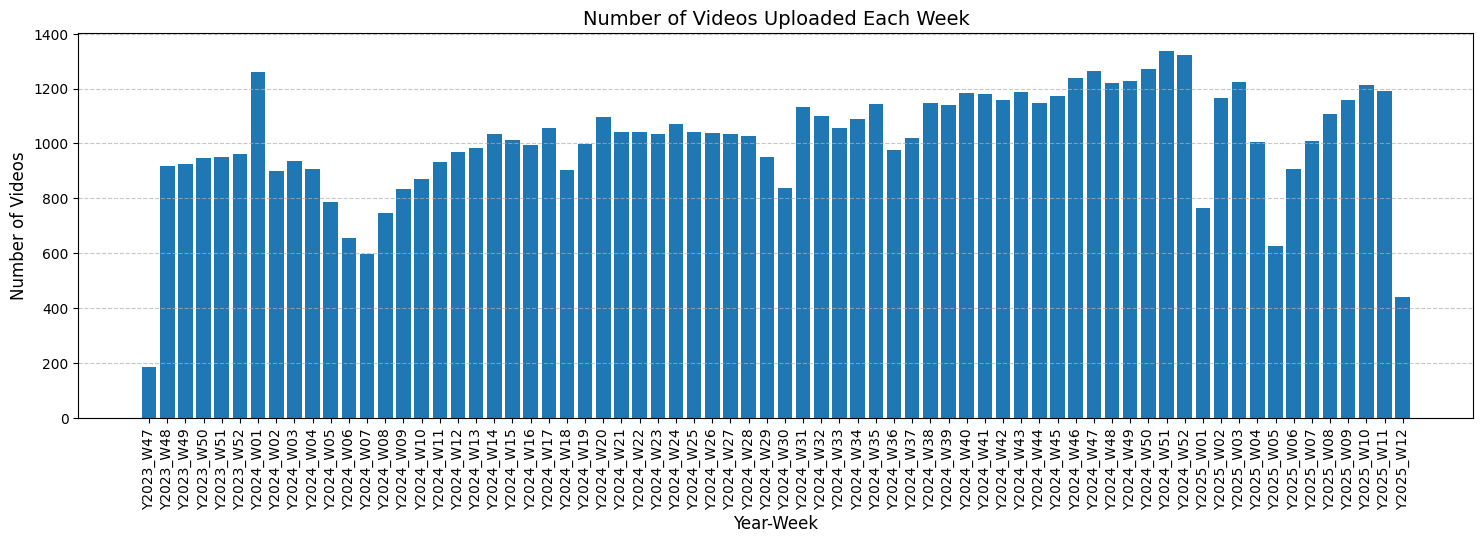
\includegraphics[width=1\linewidth]{img/21127739/num_video_per_week.png}
    \caption{Biểu đồ phân bố số lượng video được đăng tải theo các tuần trong năm}
    \label{fig:num_video_per_week}
\end{figure}

\subsubsection{Chọn top video hàng tuần để phân tích nội dung} \label{subsubsec:top_20_percent_video}

\paragraph{Mục tiêu:} 
Để tập trung phân tích sâu vào nội dung (transcript, món ăn, địa điểm) của các video tiềm năng nhất, nhóm quyết định chỉ xử lý một tập con các video nổi bật.

\paragraph{Tiêu chí lựa chọn:}
Nhóm đề xuất một \textbf{độ đo đánh giá} cho mỗi video dựa trên các chỉ số thống kê có sẵn trong tập dữ liệu, với \textbf{trọng tâm là số lượt xem} (\texttt{statsV2.playCount}). Cụ thể, độ đo này là \textbf{tổng có trọng số của lượt xem và các chỉ số tương tác} khác (như lượt thích, bình luận, chia sẻ) \textbf{sau khi được chuẩn hóa} để đảm bảo tính công bằng giữa các chỉ số. Mức độ đóng góp của mỗi chỉ số thống kê vào độ đo đánh giá như sau:
\begin{itemize}
    \item \texttt{statsV2.playCount} (lượt xem): 40\%.
    \item \texttt{statsV2.diggCount} (lượt thích): 25\%.
    \item \texttt{statsV2.shareCount} (lượt chia sẻ): 15\%.
    \item \texttt{statsV2.commentCount} (lượt bình luận): 10\%.
    \item Tỷ lệ tương tác: 10\%.
\end{itemize}

\paragraph{Quy trình:}
Tập dữ liệu bao gồm dữ liệu từ 70 tuần (xem Hình~\ref{fig:num_video_per_week}). Trong mỗi tuần, ta chọn ra \textbf{20\% số video có điểm số đánh giá cao nhất}. Tuy nhiên, để đảm bảo đủ dữ liệu cho phân tích, nếu 20\% số video ít hơn 100, thì ta sẽ lấy \textbf{tối thiểu 100 video} có điểm số cao nhất trong tuần đó.

\paragraph{Kết quả:}
Tạo ra một tập dữ liệu con chứa khoảng \textbf{14252 video} nổi bật nhất theo từng tuần, sẵn sàng cho các bước trích xuất nội dung tốn kém hơn về mặt tính toán (như gọi API).

\subsubsection{Trích xuất nội dung audio thành văn bản (Audio Transcription)} \label{subsubsec:transcript}

\noindent
Quy trình này được thực hiện trong file \texttt{03\_FE\_01\_01-Transcribe\_audio\_colab.ipynb} và bao gồm các bước:
\begin{enumerate}
    \item \textbf{Tái tạo URL:} Xây dựng lại URL của video TikTok từ \texttt{author.uniqueId} và \texttt{video.id} theo định dạng: \texttt{https://www.tiktok.com/@{author\_id}/video/{video\_id}}.
    
    \item \textbf{Tải audio}: Sử dụng thư viện \texttt{yt-dlp} kết hợp với \texttt{FFmpeg} để tải về \textbf{chỉ phần âm thanh} từ URL video TikTok. Audio được chuyển đổi sang định dạng WAV và lưu vào thư mục \texttt{AUDIO\_FOLDER}.
    
    \item \textbf{Chuyển đổi audio thành văn bản}: Sử dụng Gemini API (mô hình \texttt{gemini-2.0-flash}) để chuyển audio thành transcript. Dữ liệu âm thanh (file \texttt{.wav}) được đọc dưới dạng bytes và gửi kèm một \textbf{prompt} yêu cầu:
    \begin{itemize}
        \item Chuyển đổi \textbf{giọng nói tiếng Việt} trong audio thành văn bản (transcript).
        
        \item Rút ra 3 ý chính (takeaways) từ nội dung.
        
        \item Kiểm tra sự tồn tại của câu kêu gọi hành động (Call to Action - CTA).
        
        \item Kiểm tra sự tồn tại của yếu tố gây tò mò (Curiosity Gap).
        
        \item Trả về kết quả dưới dạng JSON với các trường: \texttt{transcript}, \texttt{takeaways}, \texttt{has\_call\_to-\\\_action}, \texttt{has\_curiosity\_gap}. Nếu không có giọng nói, trả về \texttt{None}.
    \end{itemize}
    
    \item \textbf{Lưu kết quả:} Kết quả JSON trả về từ API được lưu vào file \texttt{\{video\_id\}.json} trong thư mục \texttt{TRANSCRIPT\_FOLDER}. Một danh sách các \texttt{video\_id} đã xử lý được lưu lại trong file \texttt{transcribed\_video\_ids.txt} để tránh xử lý lại. 
    
    \item \textbf{Quản lý giới hạn API:} Để tránh vượt quá giới hạn lượt gọi của mỗi API, nhóm \textbf{sử dụng luân phiên} nhiều API key khác nhau. Mỗi API key được sử dụng cho \textbf{14 yêu cầu liên tiếp}, sau đó chuyển sang API key tiếp theo.
\end{enumerate}

\subsubsection{Trích xuất thông tin món ăn và địa điểm}

\noindent
Quy trình này được thực hiện trong file \texttt{03\_FE\_02\_01-Extract\_food\_location\_colab.ipynb} và dựa trên kết quả từ bước trước:
\begin{enumerate}
    \item \textbf{Dữ liệu đầu vào:} Sử dụng cột \texttt{desc} (mô tả gốc) và cột \texttt{transcript} (văn bản từ audio) của các video đã được xử lý ở Mục~\ref{subsubsec:transcript} để trích xuất thông tin về món ăn, thành phố, và quận/huyện.
    
    \item \textbf{Gọi Gemini API:} Tiếp tục sử dụng mô hình \texttt{gemini-2.0-flash}. Một \textbf{prompt} mới được thiết kế để yêu cầu mô hình phân tích nội dung \texttt{desc} và \texttt{transcript}, sau đó trích xuất:
    \begin{itemize}
        \item Danh sách các món ăn được đề cập (\texttt{foods}: list of strings).

        \item Tên thành phố (\texttt{city}: string).
        
        \item Tên quận/huyện (\texttt{district}: string).
        
        \item Prompt cũng yêu cầu mô hình trả về \texttt{None} cho các trường nếu video không thuộc chủ đề ẩm thực.
        
        \item Kết quả phải trả về đúng \textbf{định dạng JSON}.
    \end{itemize}

    \item \textbf{Lưu kết quả:} Kết quả JSON chứa thông tin món ăn và địa điểm được lưu vào file \texttt{\{video\_id\}.json} trong thư mục \texttt{new\_food\_location}. Tương tự, một danh sách các video đã xử lý được theo dõi trong file \texttt{preprocessed\_video\_ids.txt}.
    
    \item \textbf{Quản lý giới hạn API:} Nhóm cũng sử dụng nhiều API key khác nhau để \textbf{tránh vượt quá giới hạn lượt gọi}. Mỗi API key được sử dụng cho \textbf{14 yêu cầu liên tiếp}, sau đó chuyển sang API key tiếp theo.
\end{enumerate}

\subsubsection{Trích xuất đặc trưng về thể loại của video}

Và đặc trưng quan trọng cuối cùng mà ta cần rút trích là \textbf{thể loại của video}. Đây là các đặc trưng được sử dụng trực tiếp trong quá trình xây dựng công cụ hỗ trợ viết kịch bản cho video TikTok. Quy trình này sẽ được trình bày chi tiết trong Chương~\ref{sec:scriptwriting}.

